\section{Experiments and Results}
\label{sec:experiments}

We evaluate our neuron population reconstruction approach in an ultra-scale OM image slice of a mouse brain in dimension of $25397\times 18516\times 869$ ($761$ GB), as Fig.~\ref{fig:brain} shows.
%
The image was captured by the VISoR imaging system~\cite{Wang2019} at a physical resolution of $0.5 \times0.5 \times 0.5$ \SI{}{\micro\metre}$^3$ per voxel. 
%
The image intensity is in 16-bit dynamic range, which preserves sufficient signal details.
In order to evaluate our PLNPR method for neuronal reconstruction in local blocks, we first conduct extensive experiments on the VISoR-40 dataset which we build and the BigNeuron dataset~\cite{peng2015}. 
%
Then we test our UltraNPR algorithm for neuronal population reconstruction in a slice of the mouse brain image.

\subsection{Evaluation of PLNPR on VISoR-40 Dataset}
\label{sec:exp_PLNPR_VISoR}

\subsubsection{VISoR-40 Dataset}
Though many neuron tracing techniques have been proposed, no dataset of OM images has been built for dense neuronal population reconstruction.
We construct a neuron image dataset ``VISoR-40'' (available at \url{https://braindata.bitahub.com/Neuronal_population_reconstruction.html}) for evaluation. 
The VISoR-40 dataset consists of 40 OM image blocks cropped from the mouse brain image. The dimension of the blocks ranges from $419 \times1197 \times 224$ to $869 \times1853 \times 575$.
%
We randomly select $32$ blocks for progressively training the segmentation network without manual annotation in our PLNPR.
%
The remaining 8 blocks with manual annotations are used as the test data.
Each image block for test was first labeled manually and independently by two experts. Then, by cross-checking their results, their agreed annotations were approved by another expert to generate the final ground truth.

\subsubsection{Experimental Settings and Evaluation Metrics}


Pytorch is adopted to implement the DSN model. At each iteration of the progressive learning, the network is trained from scratch with weights initialized from a Gaussian distribution with zero-mean and variance of $ 0.01 $. The optimization is realized with the stochastic gradient descent algorithm with the Adam update rule (batch size of 1, weight decay of $ 0.0005 $, momentum of $ 0.9 $). The base learning rate is set to $ 0.001 $ and descended with the ``poly" learning rate policy (power of $ 0.9 $ and the maximum iteration number of $ 24000 $). 
%The cube size is set as $160\times 160\times 160$ considering the GPU memory limitation.

To quantitatively evaluate our method, four commonly used metrics defined in \cite{Quan2015}, including precision, recall, F-Score, and Jaccard, are computed to measure the fidelity between the reconstruction results and the ground truth. 
Their definitions are defined as follows:
\begin{flalign}
&Precission(R,G)= \frac{\vert R \cap G\vert}{\vert R\vert} = \frac{\vert TP\vert}{\vert R\vert}, & \\
&Recall(R,G) = \frac{\vert R\cap G\vert}{\vert G\vert} = \frac{\vert TP\vert}{\vert G\vert}, & \\
&F{-}Score(R,G)= \frac{2\vert R \cap G\vert}{\vert R\vert + \vert G\vert} = \frac{2\vert TP\vert}{\vert R\vert + \vert G\vert}, & \\
&Jaccard(R,G)= \frac{\vert R\cap G\vert}{\vert R\cup G\vert} = \frac{\vert TP\vert}{\vert R\cup G\vert}, &
\label{equ: metrics}
\end{flalign}
%
where $R$ denotes the set of points on the reconstructed neurons, $G$ denotes the set of neuron points in the ground truth and $TP$ denotes the set of true positive points, $|\cdot|$ denotes the number of points in a set.
%We follow the rule of determining true positive points described in~\cite{Quan2015}. 
The four metrics are first computed on each individual neuronal tree according to the manually labeled skeleton, and then averaged in a neuronal population weighted by the total length of the neuronal processes of each neuron, the same as \cite{Quan2015}.



\subsubsection{Progressive Learning}

The key idea of PLNPR is to progressively improve the performance of neuron reconstruction by making the neuron segmentation network and the conventional tracing method complementary and synergistic without using any manual annotations.
In order to demonstrate the performance improvement, four widely-used tracing methods, including APP1~\cite{Peng2011}, APP2~\cite{Xiao2013}, MOST~\cite{Wu2014} and NGPST~\cite{Quan2015}, are tested as the neuron tracing module in our framework. 
We use their implementations in the software Vaa3D~\cite{Peng2014}. 
%
Eight iterations are tested on our VISoR-40 dataset, and the improvement of neuronal population reconstruction is shown in Fig.~\ref{fig:ablation_study_plnpr}~(a).
We only show the F-Score which is widely used to reflect the overall performance of neuron reconstruction.
%
Moreover, the neuron reconstruction results on a test block at different iterations are shown in the Fig.~\ref{fig:trace_iterations}.
%
\xj{More qualitative and quantitative results are reported in the supplementary materials.}
The results show that our progressive learning strategy effectively facilitates conventional tracing methods to reconstruct more complete neuronal populations.
In addition, the performance improvement gets stable after five iterations of the progressive learning for all the tested tracing methods. 

 

\begin{figure*}[t]
	\centering
	\subfigure[]{
		\begin{minipage}[b]{0.32\linewidth}
			\centering
			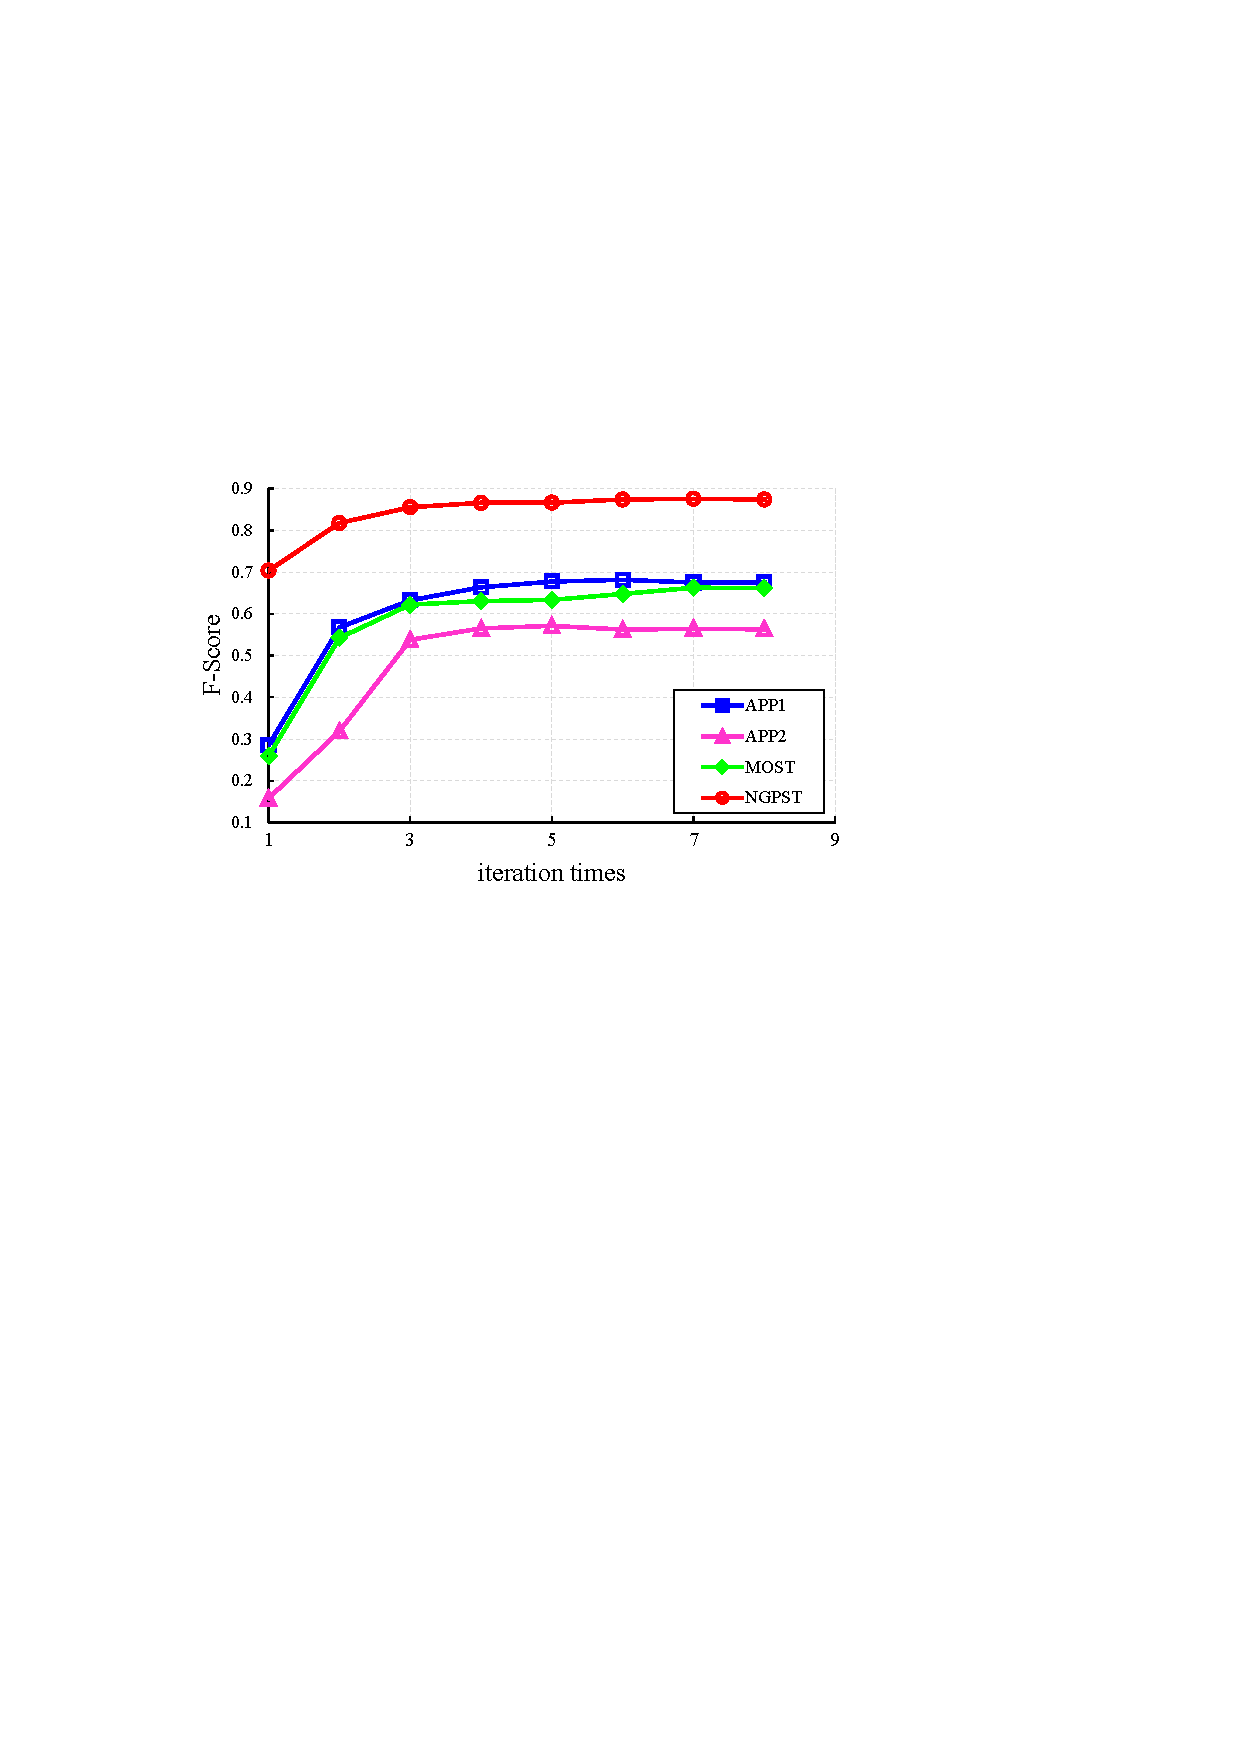
\includegraphics[height=3.7cm]{./Illustrations/trace_iterations_fscore8.pdf}
		\end{minipage}}
	\subfigure[]{
		\begin{minipage}[b]{0.32\linewidth}
			\centering
			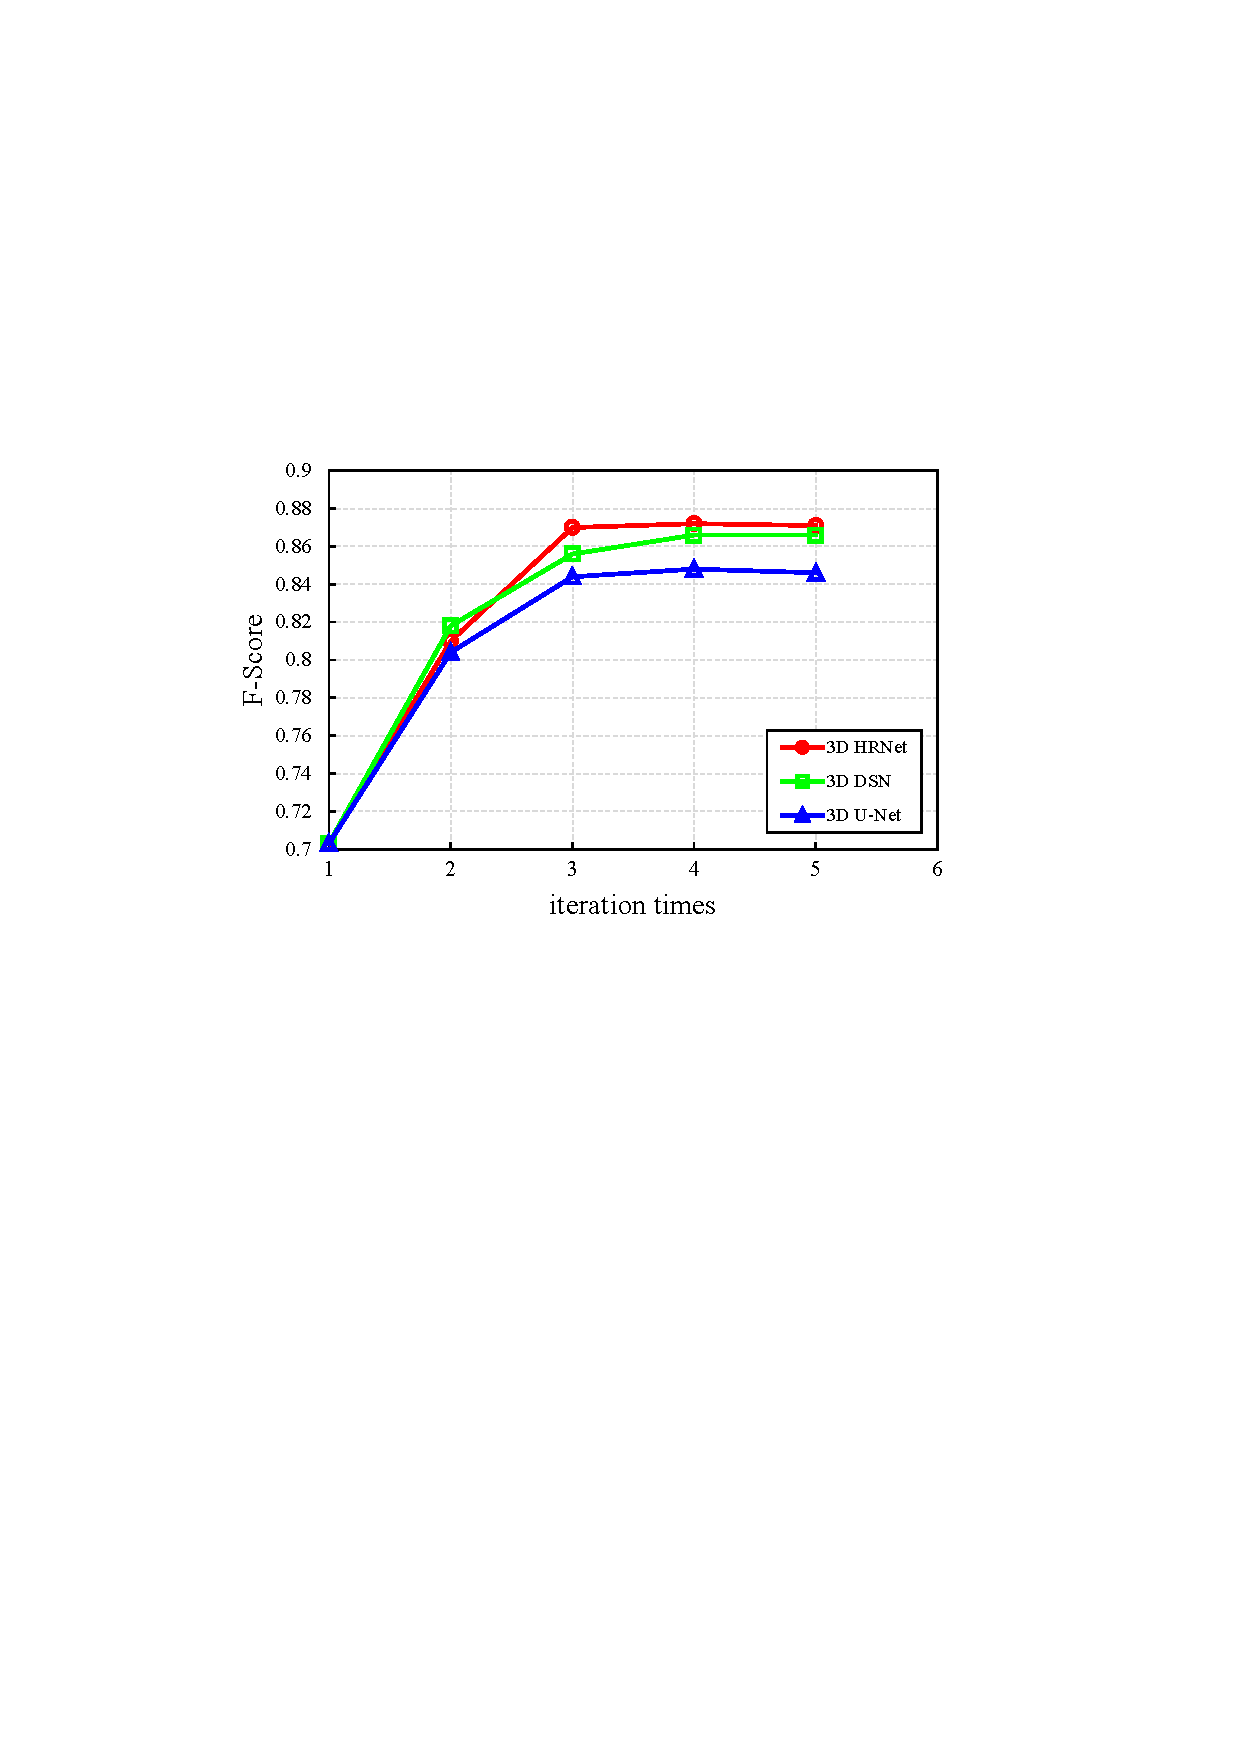
\includegraphics[height=3.7cm]{./Illustrations/trace_networks_fscore11.pdf}
		\end{minipage}}
	\subfigure[]{
		\begin{minipage}[b]{0.32\linewidth}
			\centering
			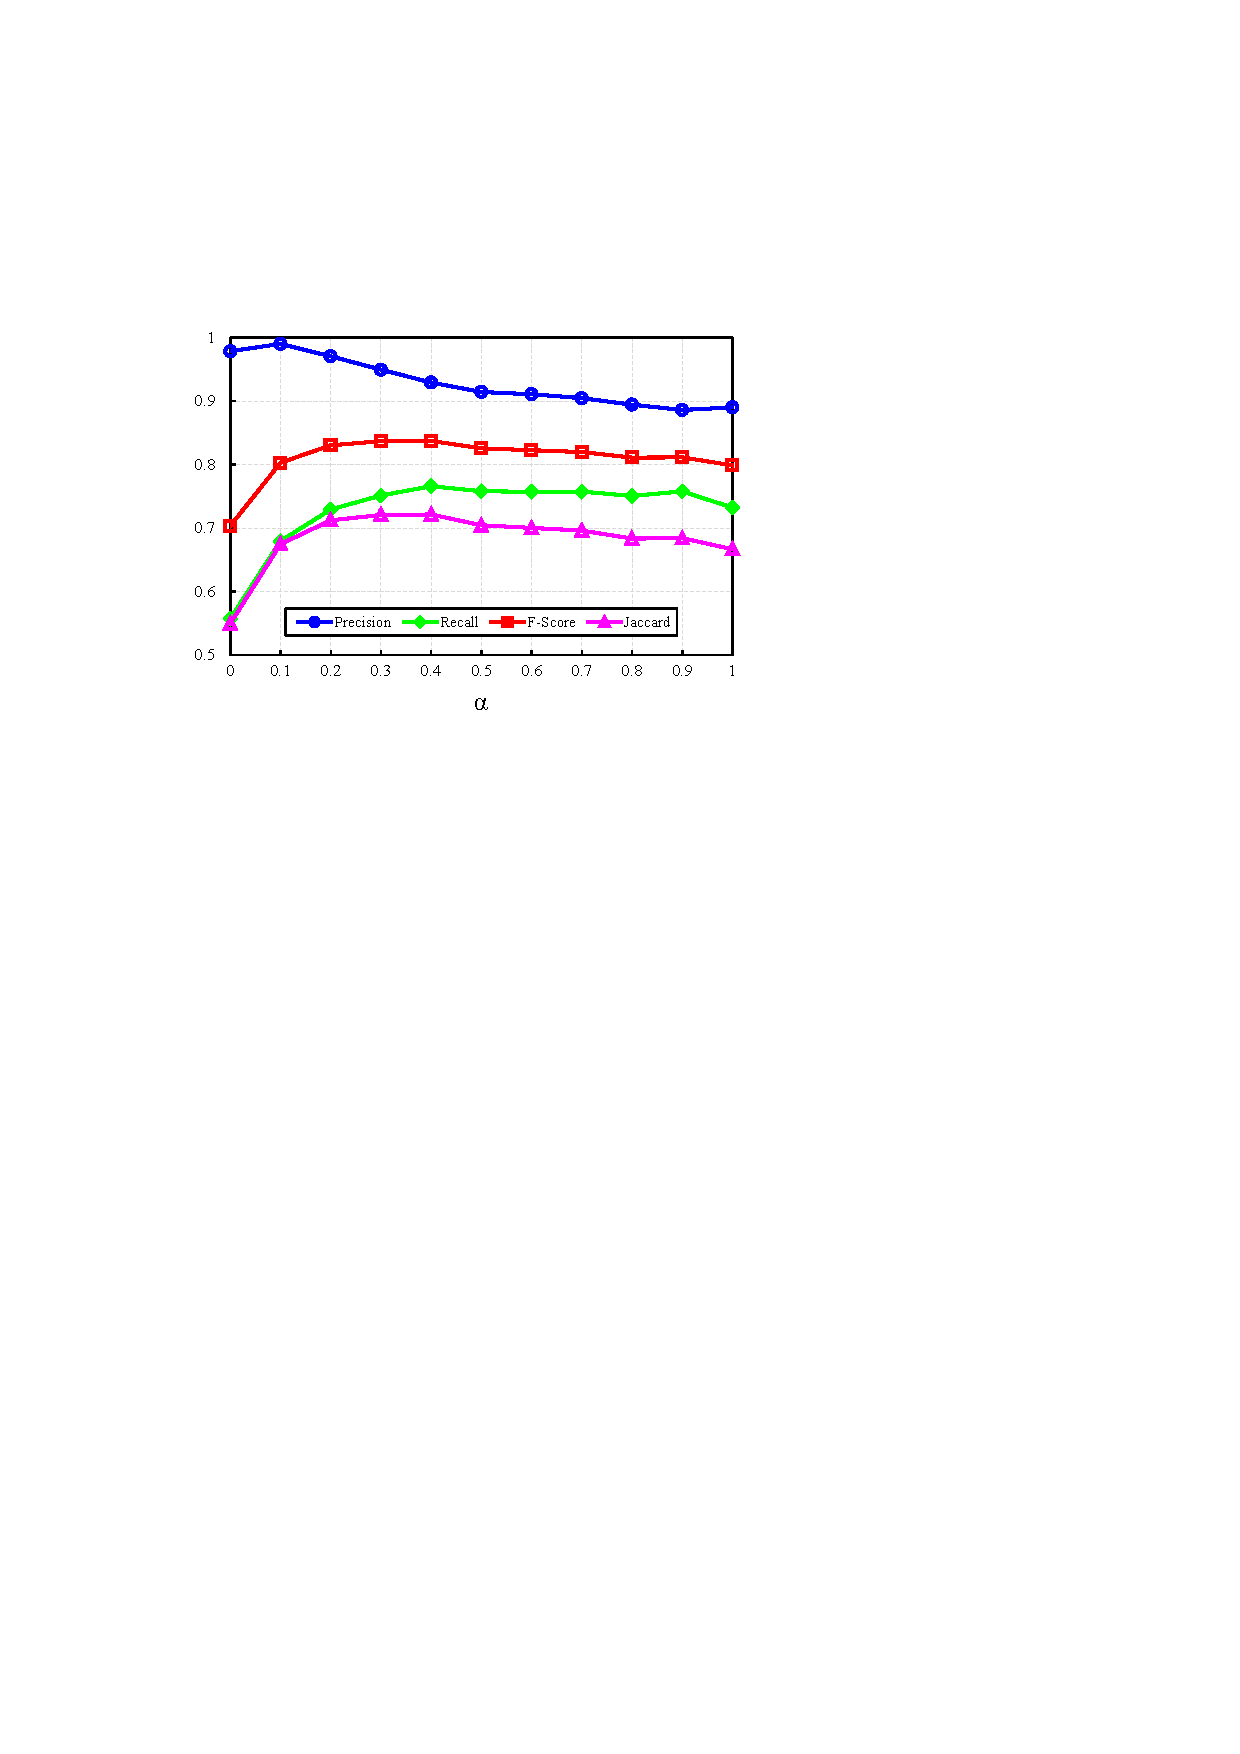
\includegraphics[height=3.7cm]{./Illustrations/weight_paprameter7.pdf}
		\end{minipage}}
	\caption{ Comparison of different parameters in our PLNPR framework on the VISoR-40 dataset.
		(a) Comparisons of neuronal population reconstruction performance at different iterations using four neuron tracing methods. 
		(b) F-Score of neuron reconstruction at five iterations using three deep segmentation networks. 
		Combining any base tracer and any one of the three neuron segmentation networks, our approach progressively improves the reconstruction performance.
		(c) Neuron reconstruction performance with different $\alpha$ in Eq.~\eqref{equ: enhance} for image enhancement.} %From left to right, the value of $\alpha$ increases from $0$ to $1$ by a step of $0.1$.
	
	\label{fig:ablation_study_plnpr}
\end{figure*}


\begin{figure}[t]
	\centering
	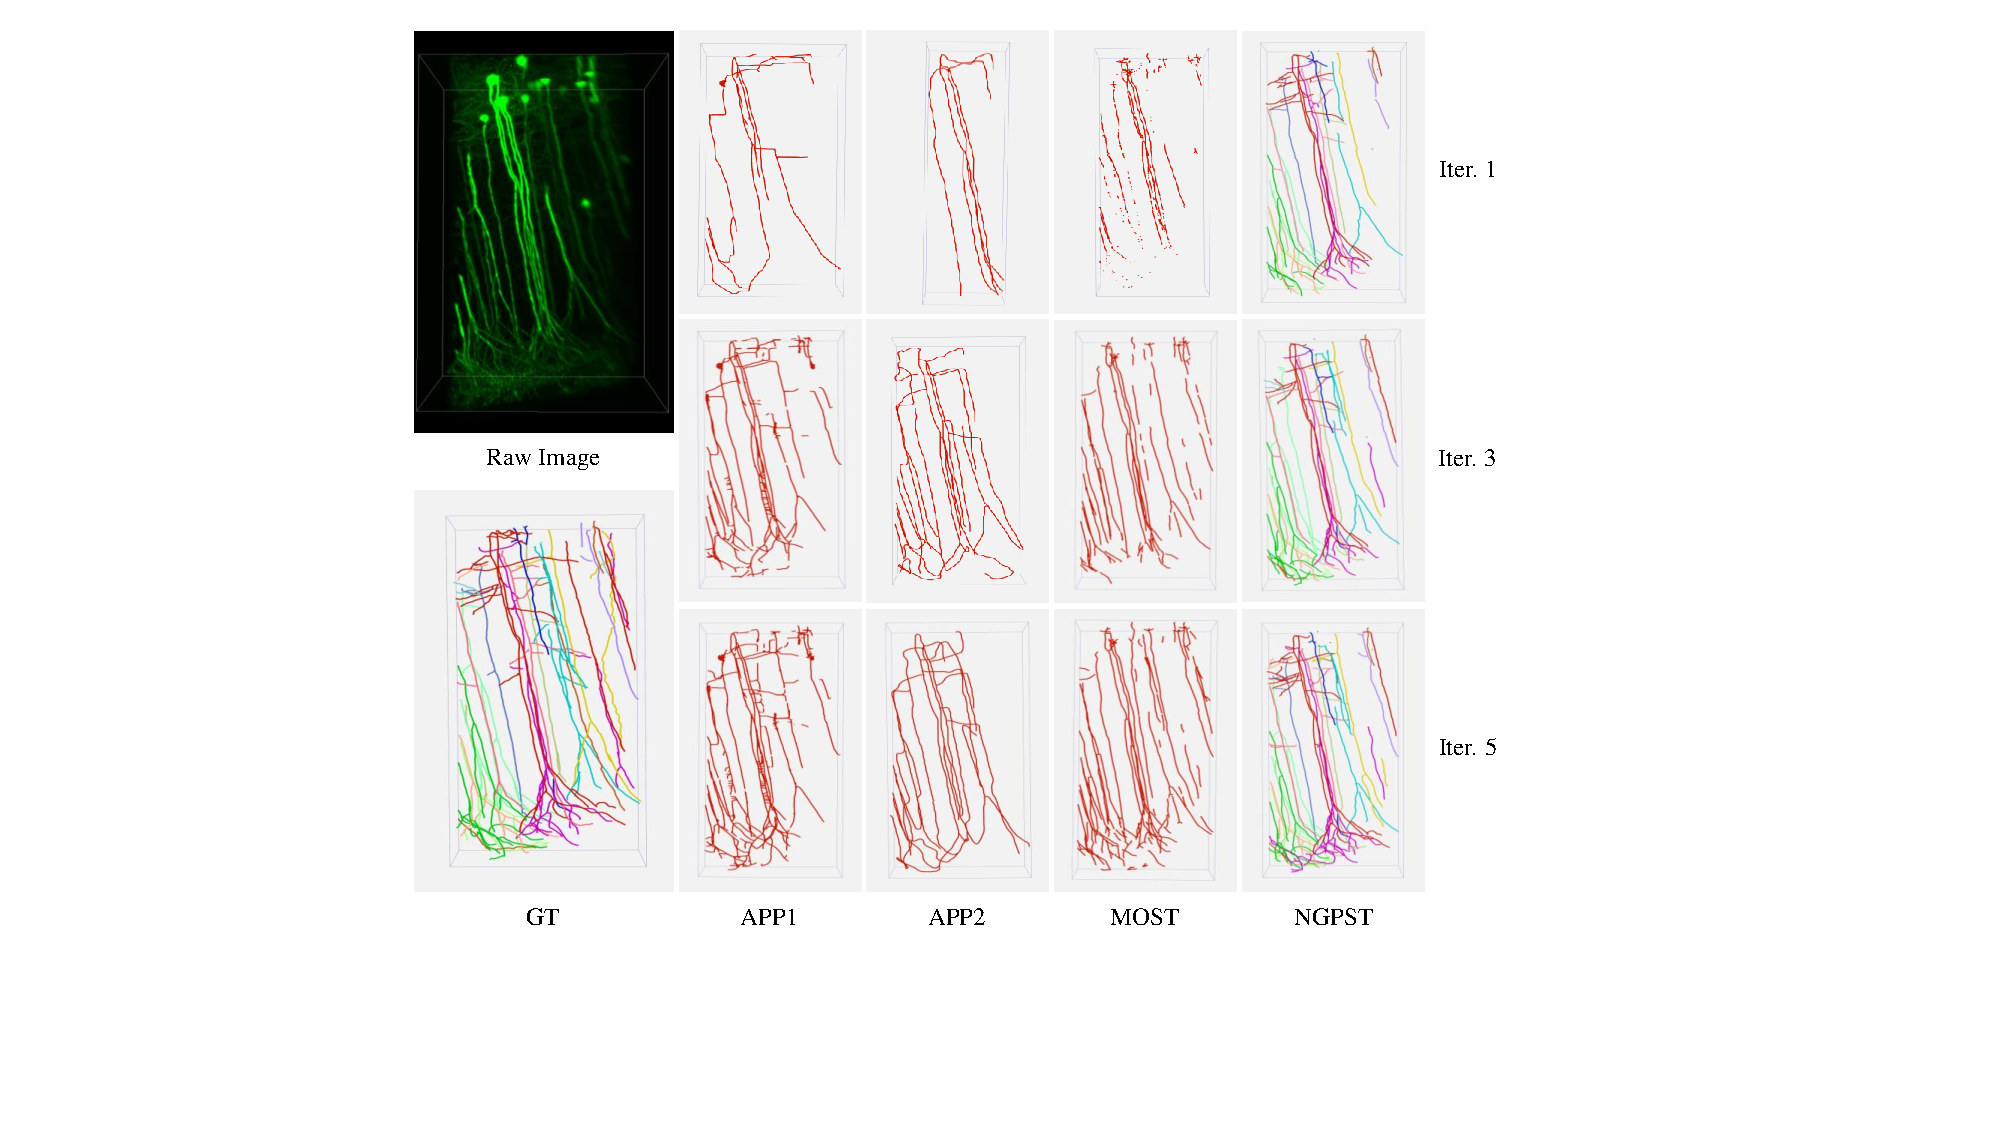
\includegraphics[width=1\columnwidth]{./Illustrations/trace_iterations3.pdf}
	\caption{Neuronal population reconstruction results of a test block at different iterations (top to bottom) using four neuron tracing methods.} 
	% APP1~\cite{Peng2011}, APP2~\cite{Xiao2013}, MOST\cite{Wu2014} and NGPST~\cite{Quan2015}.}
	\label{fig:trace_iterations}
\end{figure}

\delete{
\begin{figure}[t]
	\centering
	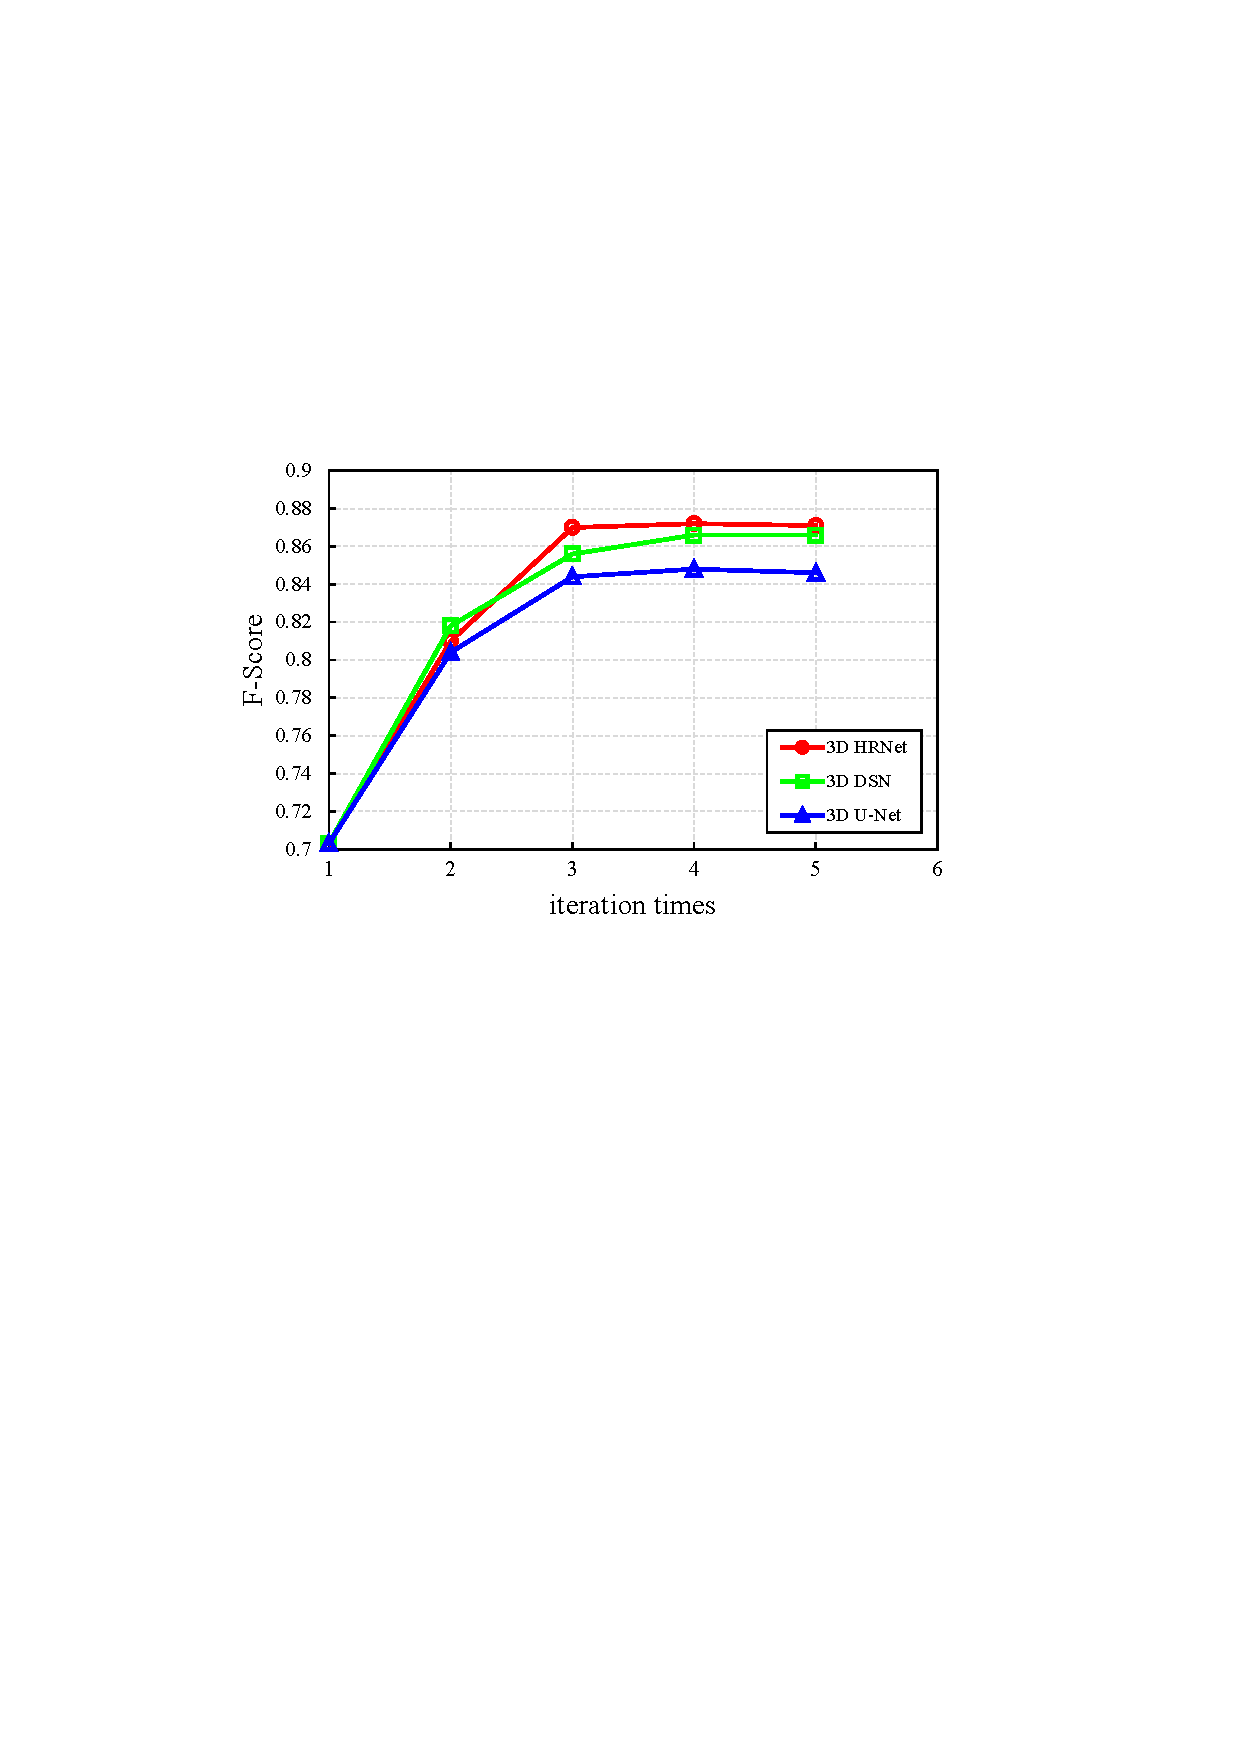
\includegraphics[width=0.8\columnwidth]{./Illustrations/trace_networks_fscore11.pdf}
	\caption{F-Score of neuron reconstruction on the VISoR-40 testing dataset at five iterations. Combining any one of the three neuron segmentation networks, our approach progressively improves the reconstruction performance.}
	\label{fig:fscore_DNNs}
\end{figure}
}


\subsubsection{Neuron Segmentation Network}

To further verify the effectiveness and robustness of our progressive learning strategy, we test three commonly-used deep segmentation networks, including 3D DSN~\cite{Dou2017}, 3D U-Net~\cite{Cicek2016} and a 3D version of HRNet~\cite{Sun2019}, for generating the neuron probability map.
Five iterations are tested on our VISoR-40 dataset, and the F-Score improvement of reconstruction results is shown in Fig.~\ref{fig:ablation_study_plnpr}~(b). 
%
It can be seen that our PLNPR algorithm effectively improves the neuron reconstruction performance by combining any one of the three neuron segmentation networks.
Consequently, the segmentation network and traditional tracing method can complement and promote each other, leading to more complete neuron reconstruction.


\subsubsection{Enhancement Parameter} 

In order to explore the influence of parameter $\alpha$ in Eq.~\eqref{equ: enhance} for image enhancement, we adopt different values for $\alpha$, and the results are shown in Fig.~\ref{fig:ablation_study_plnpr}~(c).
$\alpha=0$ means that the raw image block is directly used as input for the tracing module.
$\alpha=1$ means that only the probability maps are used as input for neuron tracing. 
It indicates that the performance is improved by combing the probability map with the raw image signal, mainly because that the probability map reflects the long-range trajectory structures while the original image signal carries more details of subtle neurites.
%Second, it can be observed our system is very robust to the parameter $\alpha$. 
%Hence, the chosen of the parameter $\alpha$ is not very demanding and the reconstruction performance can achieve significant improvement with any $\alpha >0$. 
In this paper, we empirically select $\alpha=0.1$ to reduce the influence of false positive predictions in probability maps due to the limited performance of the DNN model trained by pseudo labels and increase the robustness of the whole framework.

\delete{
\begin{figure}[t]
	\centering
	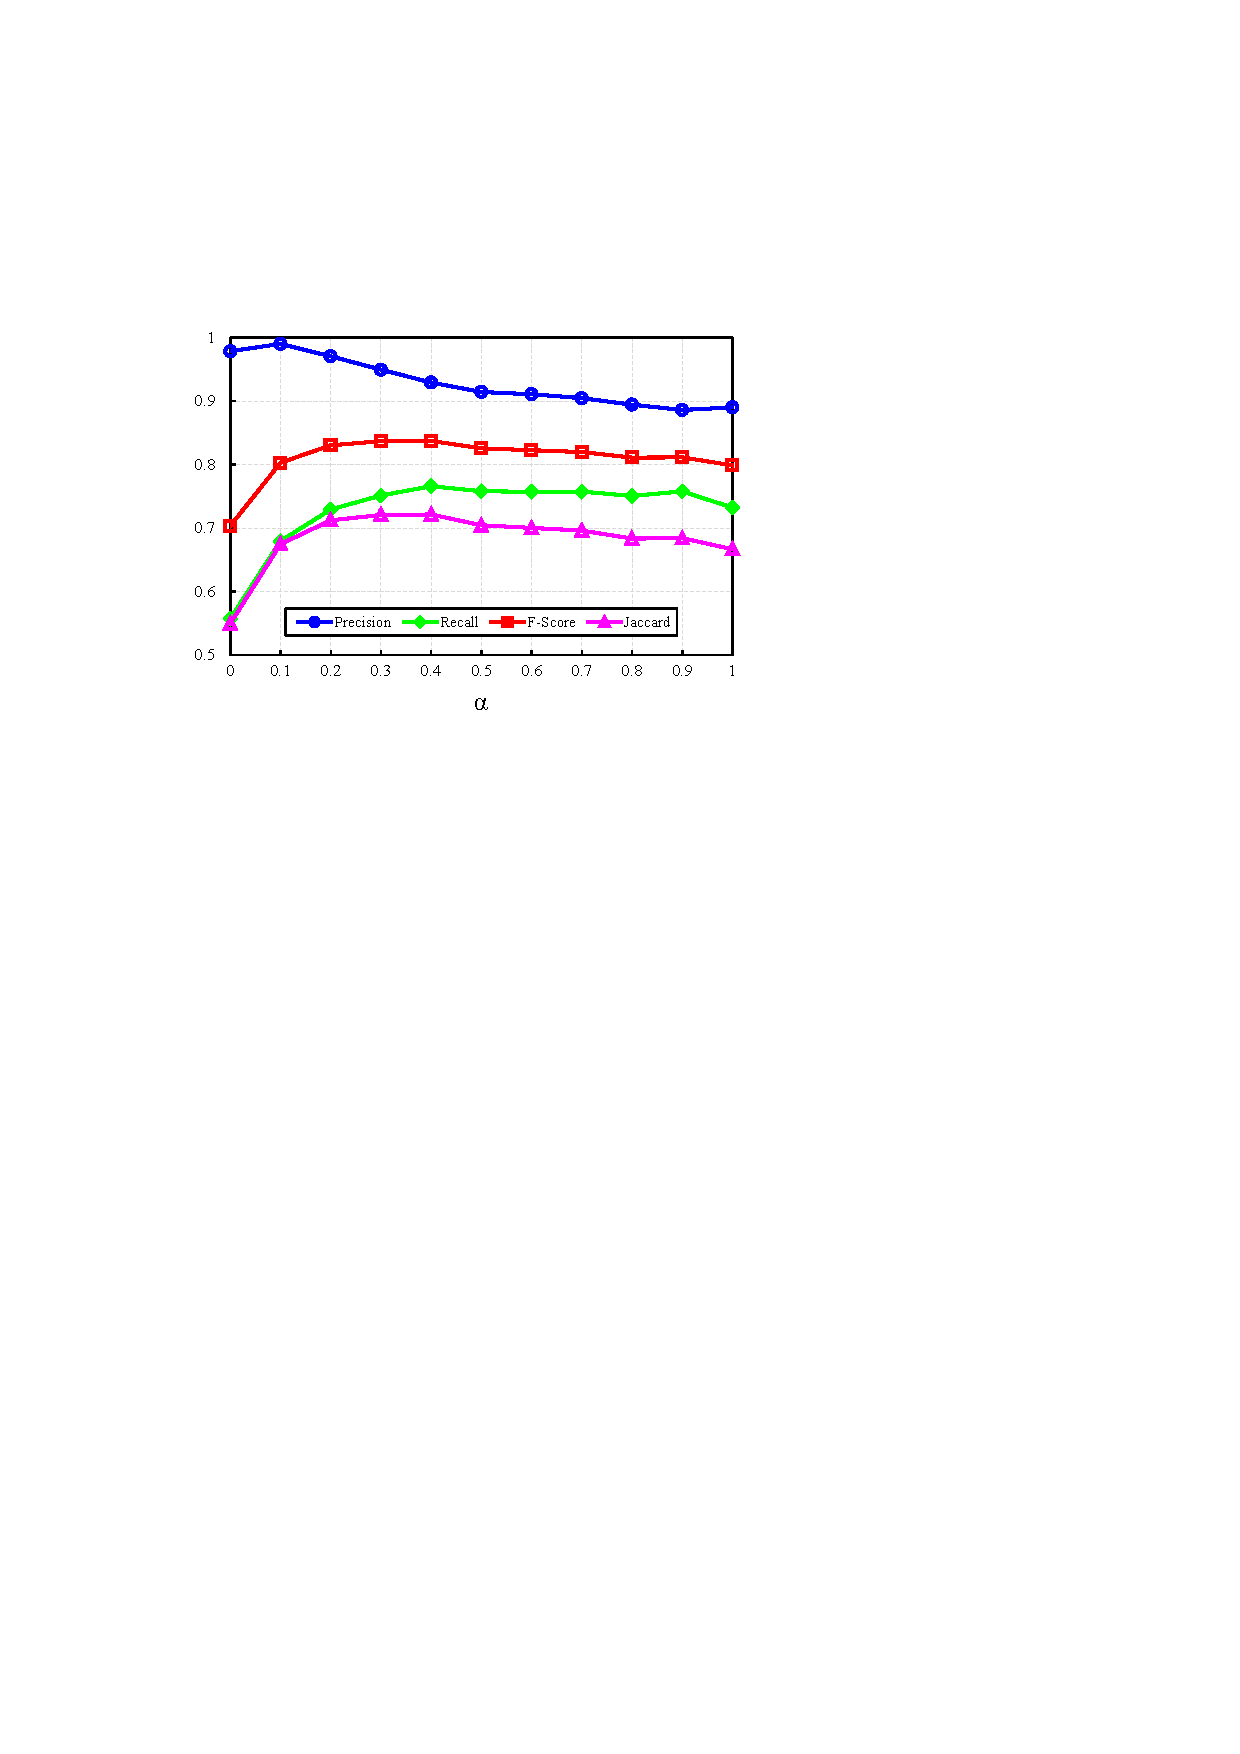
\includegraphics[width=0.8\columnwidth]{./Illustrations/weight_paprameter7.pdf}
	\caption{Neuron reconstruction performance with different $\alpha$ in Eq.~\eqref{equ: enhance} for image enhancement on the VISoR-40 test dataset. From left to right, the value of $\alpha$ increases from $0$ to $1$ by a step of $0.1$.  }
	\label{fig:weight_paprameter}
\end{figure}
}


\subsubsection{Comparison with Tracing Methods}



\begin{figure*}[t]
	\centering
	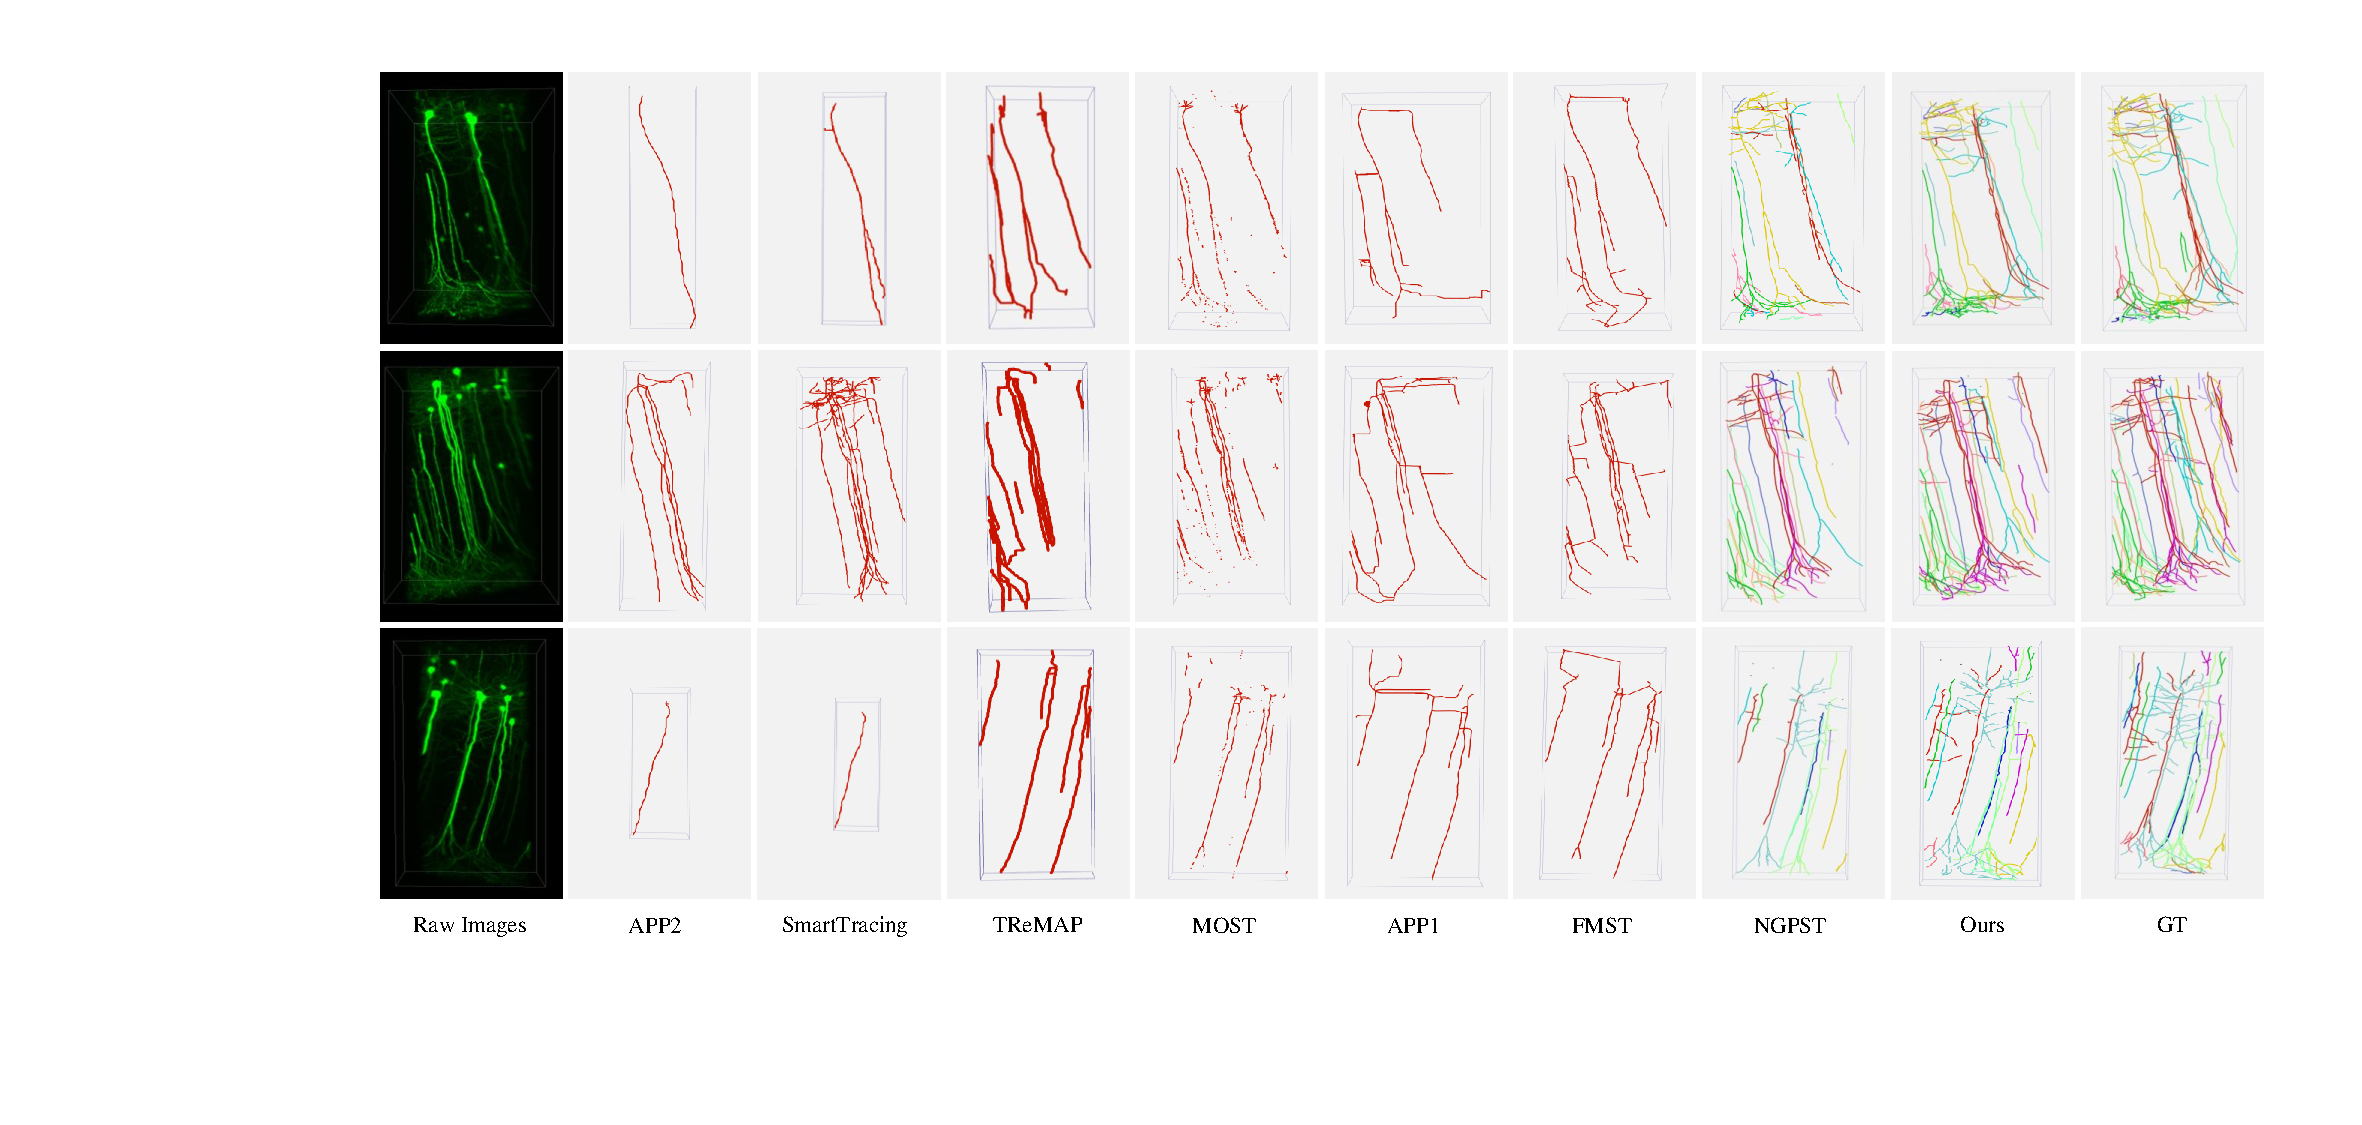
\includegraphics[width=1\textwidth]{./Illustrations/iteration3.pdf}
	\caption{Comparison of neuronal population reconstruction results of three image blocks. %using neuron reconstruction methods FMST~\cite{Yang2019}, APP1~\cite{Peng2011}, APP2~\cite{Xiao2013}, SmartTracing~\cite{Chen2015}, MOST~\cite{Wu2014}, NGPST~\cite{Quan2015} and our PLNPR on three test images from the VISoR-40 dataset.
%	Each row shows the reconstruction results generated by different methods for a test image. The first column shows the raw images, while the last column shows the ground truth (GT). Each of the remaining columns shows the reconstruction result using the corresponding tracing method. 
Our PLNPR method reconstructs more complete and accurate neurons compared to other methods. 
	}
	\label{fig:compare_VISoR}
\end{figure*}



\begin{table*}[th]
	\centering
	\caption{Performance comparison with different methods for neuronal population reconstruction on the VISoR-40 dataset.}
	\label{table:compare_VISoR}
	\begin{tabular}{lcccc}
		\toprule
		Method & Precision & Recall & F-Score & Jaccard\\
		\midrule
		%\hline
		APP2~\cite{Xiao2013}
		& \textbf{0.980} & 0.091 & 0.157 & 0.091\\
		SmartTracing~\cite{Chen2015}
		& 0.961 & 0.133 & 0.205 & 0.128\\
		TReMAP~\cite{Zhou2016}
		& 0.917 & 0.147 & 0.253 & 0.145\\
		MOST~\cite{Wu2014}          
		& 0.969 & 0.151& 0.258& 0.151\\
		APP1~\cite{Peng2011}
		& 0.935 & 0.169 & 0.284 & 0.167\\
		FMST~\cite{Yang2019}
		& 0.884 & 0.179 & 0.296 &  0.176\\
		NGPST~\cite{Quan2015}
		& 0.978 & 0.557& 0.703 & 0.549\\
		\midrule
		Ours
		& 0.971 & \textbf{0.801}&\textbf{0.875} & \textbf{0.781}\\
		\bottomrule
	\end{tabular}
\end{table*}

%<18-AAAI-Adaptive Graph Convolutional Neural Networks>
To prove the effectiveness of our method on neuronal population reconstruction, we compare it with seven widely used neuron tracing methods, including APP1~\cite{Peng2011},  APP2~\cite{Xiao2013}, MOST~\cite{Wu2014}, SmartTracing~\cite{Chen2015}, NGPST~\cite{Quan2015}, TReMAP~\cite{Zhou2016} and  FMST~\cite{Yang2019}.
The parameters of these tracing methods are manually adjusted for each image block to get the optimal performance in our experiments.
%
We utilize NGPST with 3D DSN enhancement as ``Ours''. Note that the segmentation network in our approach is trained progressively on the VISoR-40 dataset in the training stage. We use the trained model directly at the test stage for evaluation. 
%
Table~\ref{table:compare_VISoR} compares the quantitative results of different methods with regard to the four metrics including precision, recall, F-Score, and Jaccard.
%
It shows that our method makes a significant improvement on the overall performance compared with other methods.
Though APP2 achieves the highest precision, the reconstructed neurons are significantly sparser than others. 
%
Fig.~\ref{fig:compare_VISoR} shows the neuronal populations reconstructed from three test image blocks.
Compared with other methods, our PLNPR is superior in both sparse and dense neurons.
Conventional tracing methods~\cite{Peng2011, Xiao2013, Wu2014, Zhou2016} and learning-based methods~\cite{Chen2015, Yang2019} tend to extract the main trunk of neurons, while missing a large portion of subtle neurites. 
Therefore, these methods have very high precision but significantly lower recall.
Although NGPST~\cite{Quan2015} achieves better performance of neuronal population reconstruction compared with other single-neuron tracing methods, it still remains difficult to extract subtle neuron voxels for NGPST by using hand-crafted features.
%
In comparison, our method benefits from the progressively trained segmentation network, and reconstructs more complete neurons from challenging blocks, even there exhibit noises, low contrast, and blending of fluorescence in the blocks.


\subsection{Evaluation of PLNPR on BigNeuron Dataset}
\label{sec:exp_PLNPR_BigNeuron}

\subsubsection{BigNeuron Dataset}

To validate our PLNPR method on single neuron reconstruction, we employ the BigNeuron~\cite{peng2015} dataset.
% which is a well-known community-derived neuron dataset. 
This dataset consists of about $20,000$ 3D OM images in total, acquired from a variety of species and optical imaging systems by different institutes.
%Some images have the corresponding manual annotations for evaluation.  
Unlike our VISoR-40 dataset which is built for the evaluation of neuronal population reconstruction, each block in the BigNeuron dataset only contains a single neuron or fragmented neurites.
% which are appropriate for single neuron reconstruction.
Following \cite{Li2017}, we select the same 68 images that are from a variety of species to evaluate the the performance of dense neurite reconstruction.
Manual reconstruction by experts is associated with each image. 
51 images are used for network training in \cite{Li2017} and the remaining 17 images are used for evaluation.
Note that we do not use the manual annotations in our PLNPR in training the deep neural network. 


\subsubsection{Experimental Settings}
 
 
To evaluate our PLNPR on the single neuron reconstruction, we use the DSN model pretrained on the VISoR-40 dataset as initialization and fine-tune it on the BigNeuron dataset using pseudo labels generated by NGPST~\cite{Quan2015} instead of the provided manual annotations.
%
The learning rate was initialized as $\num{1e-4}$ and decayed using the ``poly" learning rate policy with power of $0.9$. The maximum iteration number is set to $ 24000 $. 
We cropped image patches of size $160\times 160\times 8$ as input to the segmentation network since the axial dimensions are usually much lower in the images of the BigNeuron dataset than our VISoR-40 dataset.
Data augmentation by transposing the three dimensions of each training image is also performed. 


\subsubsection{Comparison on BigNeuron Dataset}

\begin{figure*}[th]
	\centering
	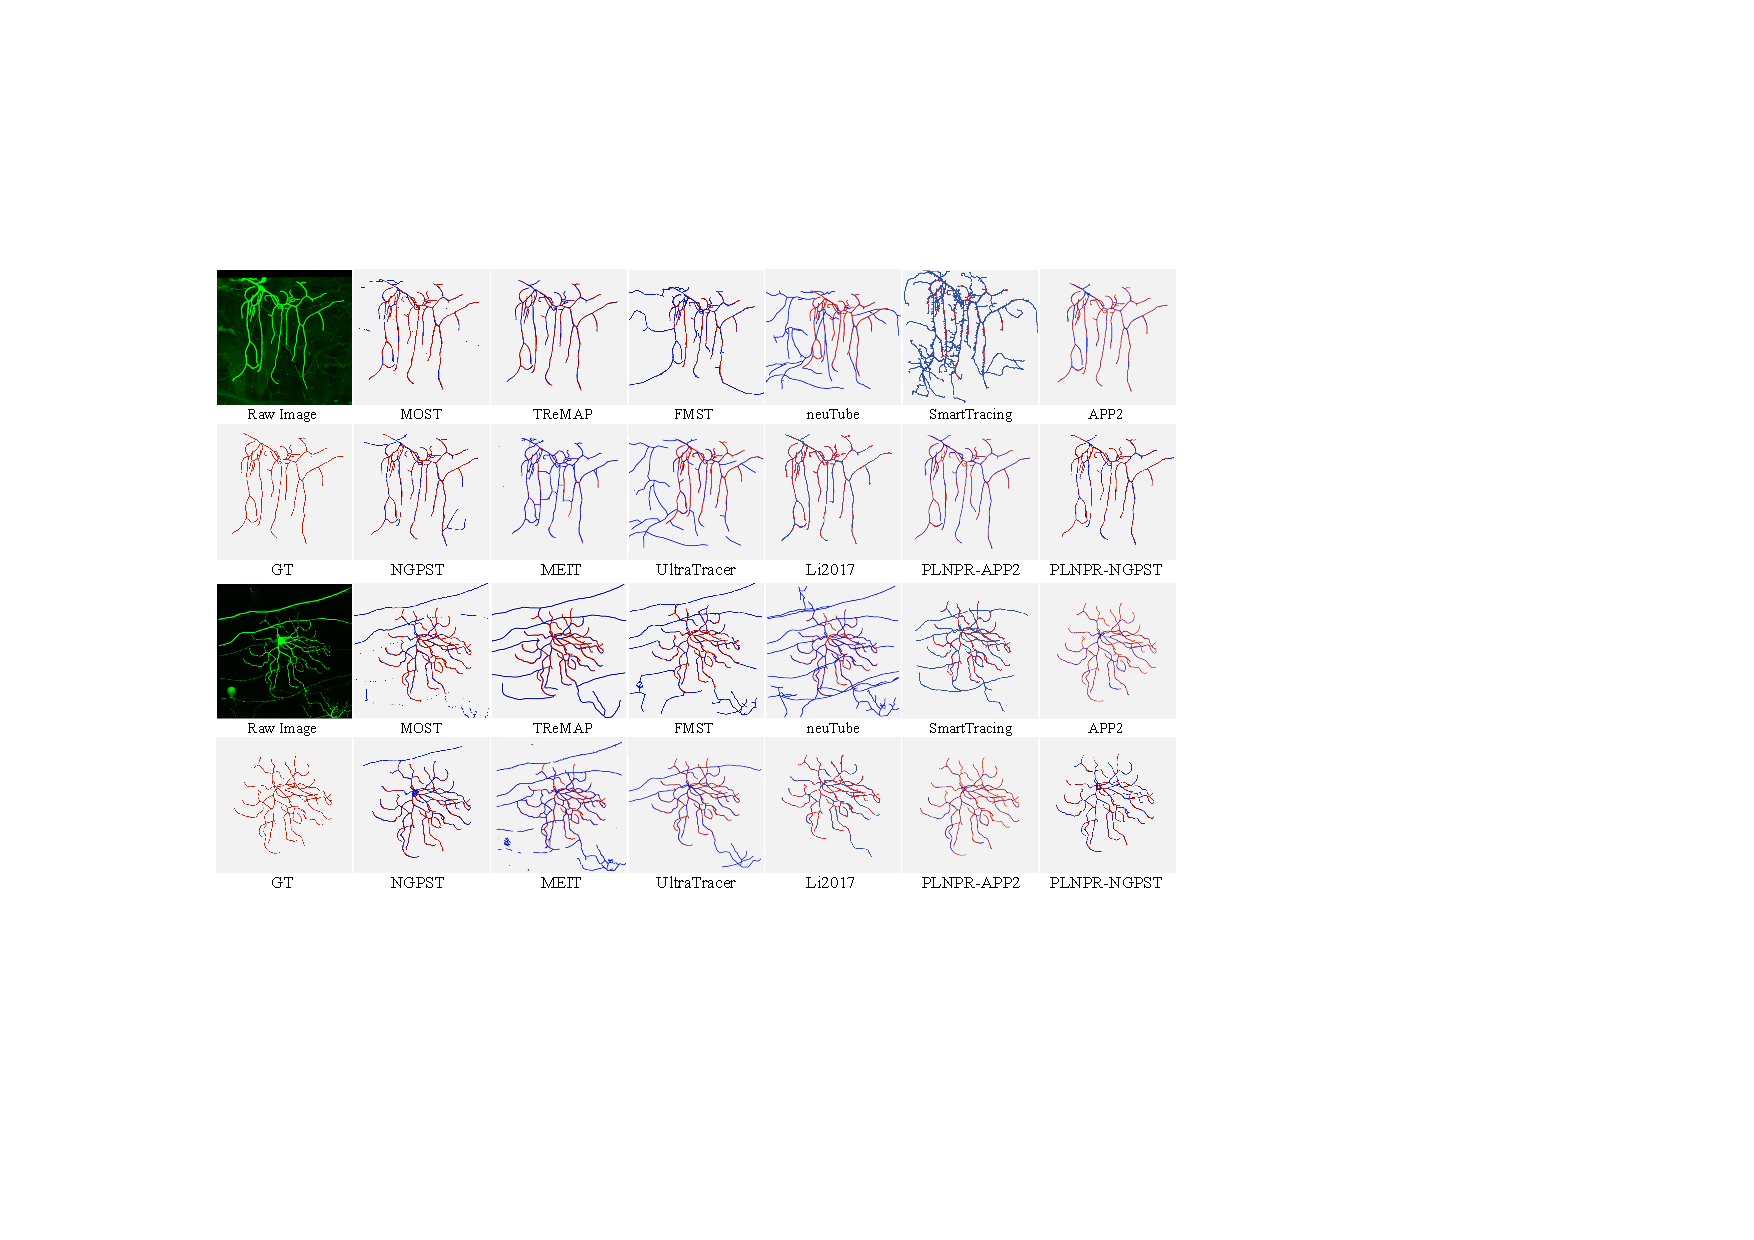
\includegraphics[width=1\textwidth]{./Illustrations/BigNeuron_comparison.pdf}
	\caption{Comparison of single neuron reconstruction results on two test images from the BigNeuron dataset.
		% using MOST~\cite{Wu2014}, FMST~\cite{Yang2019}, APP2~\cite{Xiao2013}, TReMAP~\cite{Zhou2016}, NGPST~\cite{Quan2015}, SmartTracing~\cite{Chen2015}, Li2017~\cite{Li2017} and our PLNPR on two testing images from the BigNeuron dataset.
	The reconstructed neurites are shown in blue and the corresponding ground truth (GT) are shown in red.
	Our method reconstructs more complete and accurate neurons compared to other methods.
	}
	\label{fig:compare_BigNeuron}
\end{figure*}

\begin{table*}[th]
	\centering
	\makeatletter\def\@captype{table}\makeatother
	\caption{Performance comparison for single neuron reconstruction on the BigNeuron test dataset.}
	\label{table:compare_BigNeuron}
	\begin{tabular}{lccccccc}
		\toprule
		Method & Precision & Recall & F-Score & Jaccard & ESA & DSA & PDS\\
		\midrule
		MOST~\cite{Wu2014} & 0.619 & 0.361 & 0.456 & 0.295 & 31.730 & 38.211 & 0.633\\
		FMST~\cite{Yang2019} & 0.575 & 0.629 & 0.601 & 0.429 & 17.878 & 23.459 & 0.558\\
		APP2~\cite{Xiao2013} & 0.799 & 0.492 & 0.608 & 0.437 & 13.457 & 17.923 & 0.562\\
		TReMAP~\cite{Zhou2016} & 0.771 & 0.415 & 0.539 & 0.369 & 11.269 & 17.941 & 0.539\\
		NGPST~\cite{Quan2015} & 0.710 & 0.680 & 0.695 & 0.532 & 10.168 & 14.880 & 0.587\\
		SmartTracing~\cite{Chen2015} & 0.701 & 0.648 & 0.674 & 0.508 & 8.532 & 11.609 & 0.543\\
		Li2017~\cite{Li2017} & - & - & - & - & 4.917 & \textbf{7.972} &0.461 \\
		UltraTracer~\cite{Peng2017} & \textbf{0.808} & 0.548 & 0.653 & 0.485 & 9.578 & 14.197 & 0.452 \\
		MEIT~\cite{Wang2018} &  &  &  & & 12.068 &16.578 & 0.554 \\
		\midrule
		Ours & 0.790 & \textbf{0.707} & \textbf{0.746}  & \textbf{0.595} & \textbf{4.784} & 8.309 & \textbf{0.451}\\
		\bottomrule
	\end{tabular}
\end{table*}

\begin{figure}[t]
	\centering
	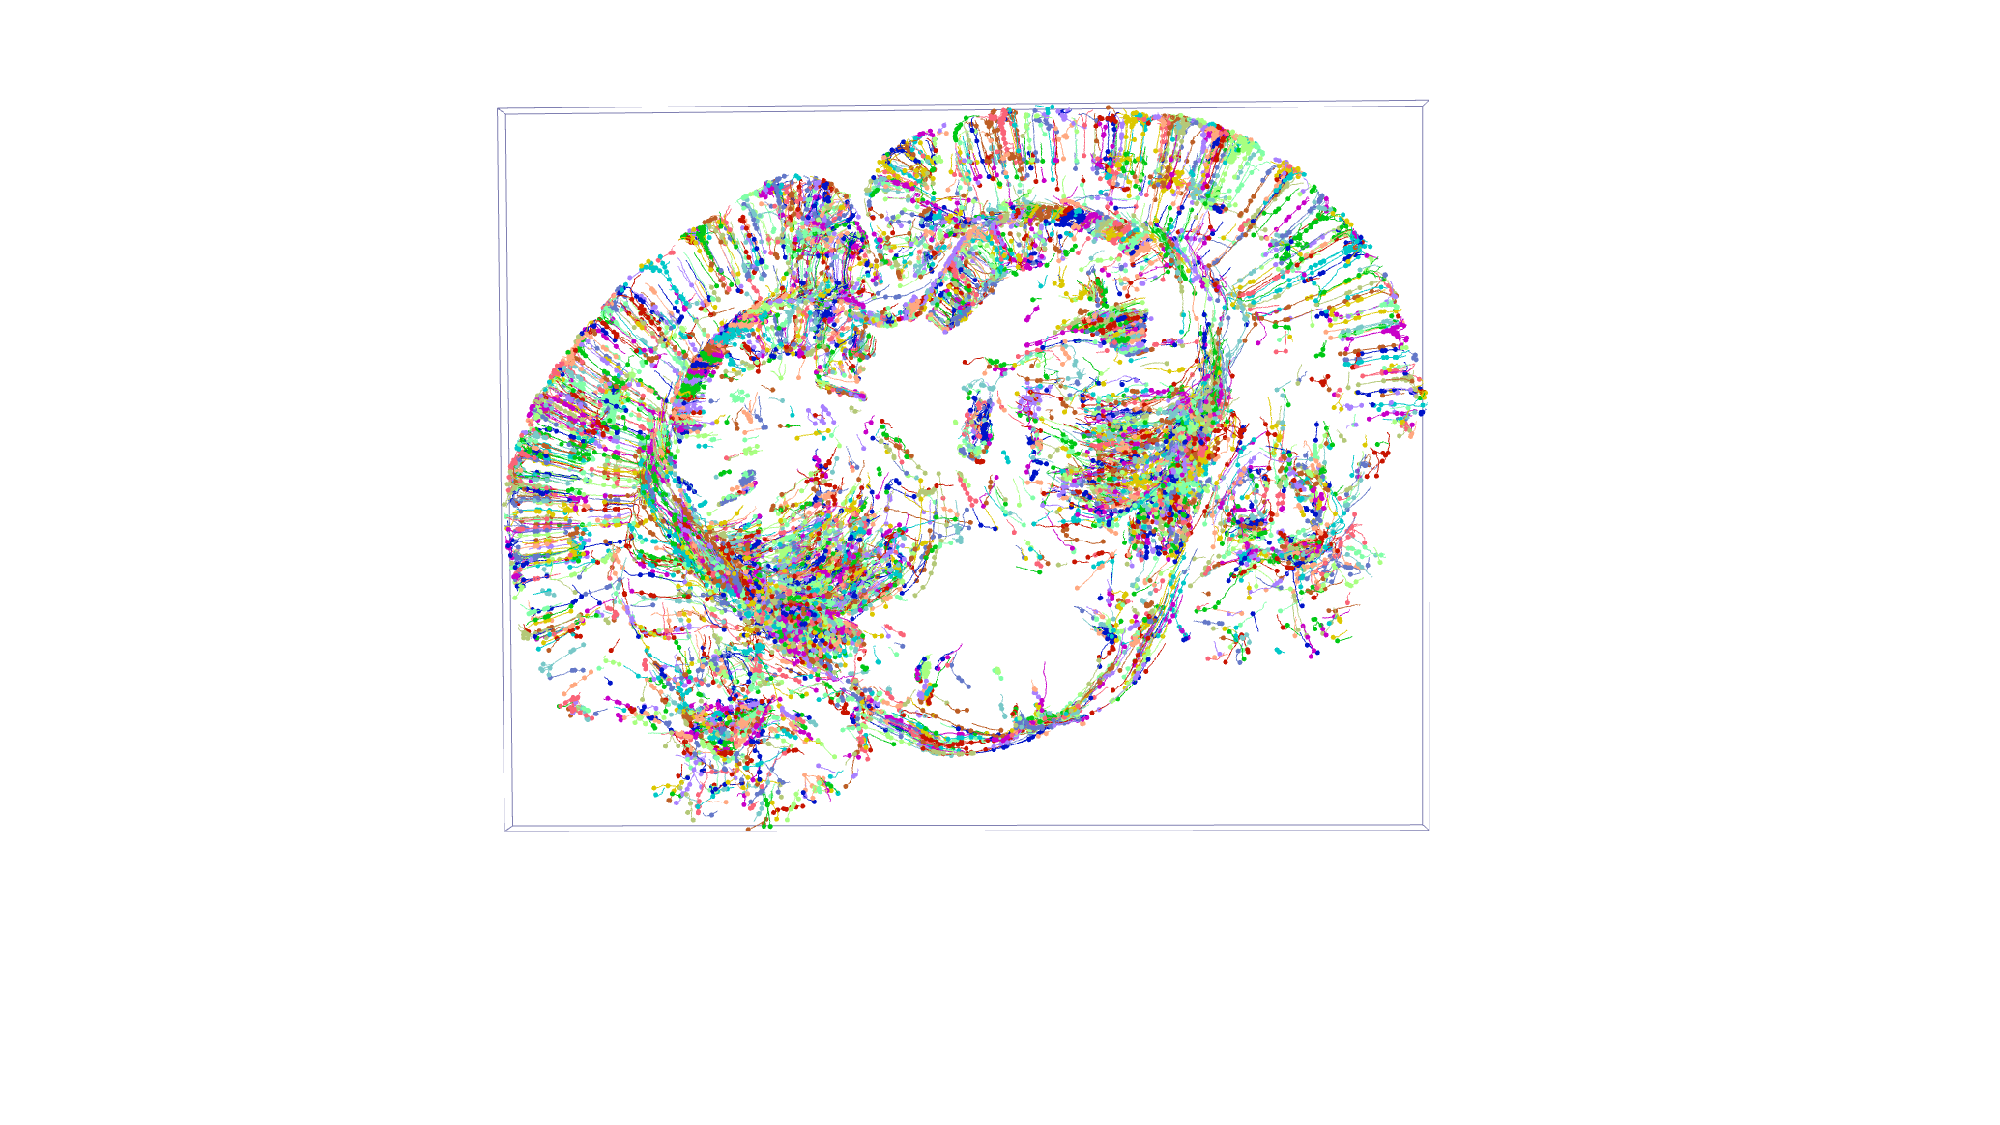
\includegraphics[width=1\columnwidth]{./Illustrations/brain_slice.pdf}
	\caption{The reconstruction result of neuronal populations in a large-scale 3D mouse brain slice using our UltraNPR method.}
	\label{fig:reconstruct_brain}
\end{figure}


On the BigNeuron dataset, we compare with seven widely used tracing methods to validate the effectiveness of our proposed method.
They are APP2~\cite{Xiao2013}, MOST~\cite{Wu2014}, SmartTracing~\cite{Chen2015}, NGPST~\cite{Quan2015}, Li2017~\cite{Li2017}, TReMAP~\cite{Zhou2016} and FMST~\cite{Yang2019} respectively.
%
The four metrics, including precision, recall, F-score, and Jaccard, are used for comparison for most methods.
However, the implementation of most learning-based tracing methods, such as~\cite{Li2017}, are not available.
In order to compare with~\cite{Li2017}, we only compare the three evaluation metrics reported in \cite{Li2017} on the same test data.
%
The three metrics defined in~\cite{Peng2010a} include the entire structure average (ESA), different structure average (DSA) and percentage of different structures (PDS).  
%
We evaluate the results obtained from different methods on the BigNeuron dataset in Table~\ref{table:compare_BigNeuron}.
The weighted averages of the ESA, DSA and PDS are calculated by setting the of each test block proportional to the neuron length identified in the corresponding manual annotation.
For these three scores, larger values indicate higher discrepancy between the tracing results and the manual reconstruction.
%
Fig.~\ref{fig:compare_BigNeuron} shows the reconstructed neurons from two test images using different methods.
%
From Table~\ref{table:compare_BigNeuron}, we can see that our method outperforms other methods on the BigNeuron dataset.
Though APP2~\cite{Xiao2013} achieves the highest precision, a large portion of subtle neurites are missing, as shown in Fig.~\ref{fig:compare_BigNeuron}.
%
Comparing with \cite{Li2017}, our PLNPR achieves comparable performance.
%
However, our method does not require any manual annotations to train the deep segmentation network.
With ever-increasing number of unlabeled neuron datasets are collected, our method could utilize them to further improve the performance of neuron reconstruction.



\subsection{Evaluation of UltraNPR on a Mouse Brain Slice}
\label{sec:exp_UltraNPR}

%\subsubsection{Experimental Settings}
To reconstruct the dense neuron population from an ultra-scale image, we divide the entire image into blocks in size of $1120\times 2048\times 869$ considering the memory and computational efficiency of our PLNPR.
%
The overlap between adjacent blocks is set to be $300$ voxels along each dimension. 
The $\delta_{ovlp}$ is set to be 10 voxels.
The $\delta_{bound}$ is set to be 70 voxels and the $\delta_{pt}$ is set to be 10 voxels for neurite fusion in Sec.~\ref{sec:fusion}.
%
It took our UltraNPR about 34 hours for deep image segmentation, 1 hour for neuron reconstruction in blocks, and 10 hours for neurite fusion to reconstruct the dense neuron population from the entire image on a cluster computer with $64$ GB of working memory and 20 NVIDIA 1080Ti GPUs.
%
As shown in Fig.~\ref{fig:reconstruct_brain}, a neuronal population which consists of $5348$ neurons is successfully reconstructed in the brain slice.


Since it is infeasible to manually annotate the dense nueron population in an ultra-scale image, quantitative evaluation of the reconstruction performance is supported.
%
However, we select four adjacent large-scale image blocks to qualitatively compare our UltraNPR with two state-of-the-art methods, UltraTracer~\cite{Peng2017} and MEIT~\cite{Wang2018}, for large-scale neuron reconstruction.
%
Fig.~\ref{fig:reconstruct_blocks} shows the neuronal populations reconstructed results.
%
MEIT~\cite{Wang2018} is designed for tracing single neuron, without separating individual neurons. 
Moreover, it fails to reconstruct the subtle dendrites due to the noises and low contrast in our challenging image.
%
\xj{Another drawback of MEIT is that many parameters have to be carefully tuned to obtain satisfied results. More results under different parameters using MEIT are shown in our supplementary files. }
% 
UltraTracer~\cite{Peng2017} achieves better performance of neuronal population reconstruction from the large-scale image. 
However, for the local regions with low signal-noise-ratio, it fails to separate individual neurons and trace complete dendrites in a dense neuron population. 
In comparison, thanks to the signal enhancement by our deep network and block propagation designed for dense neurites, our UltraNPR is more robust to reconstruct a more complete neuronal population from the low-quality image while individual neurons are continuously and smoothly traced.
 

\begin{figure*}[t]
	\centering
	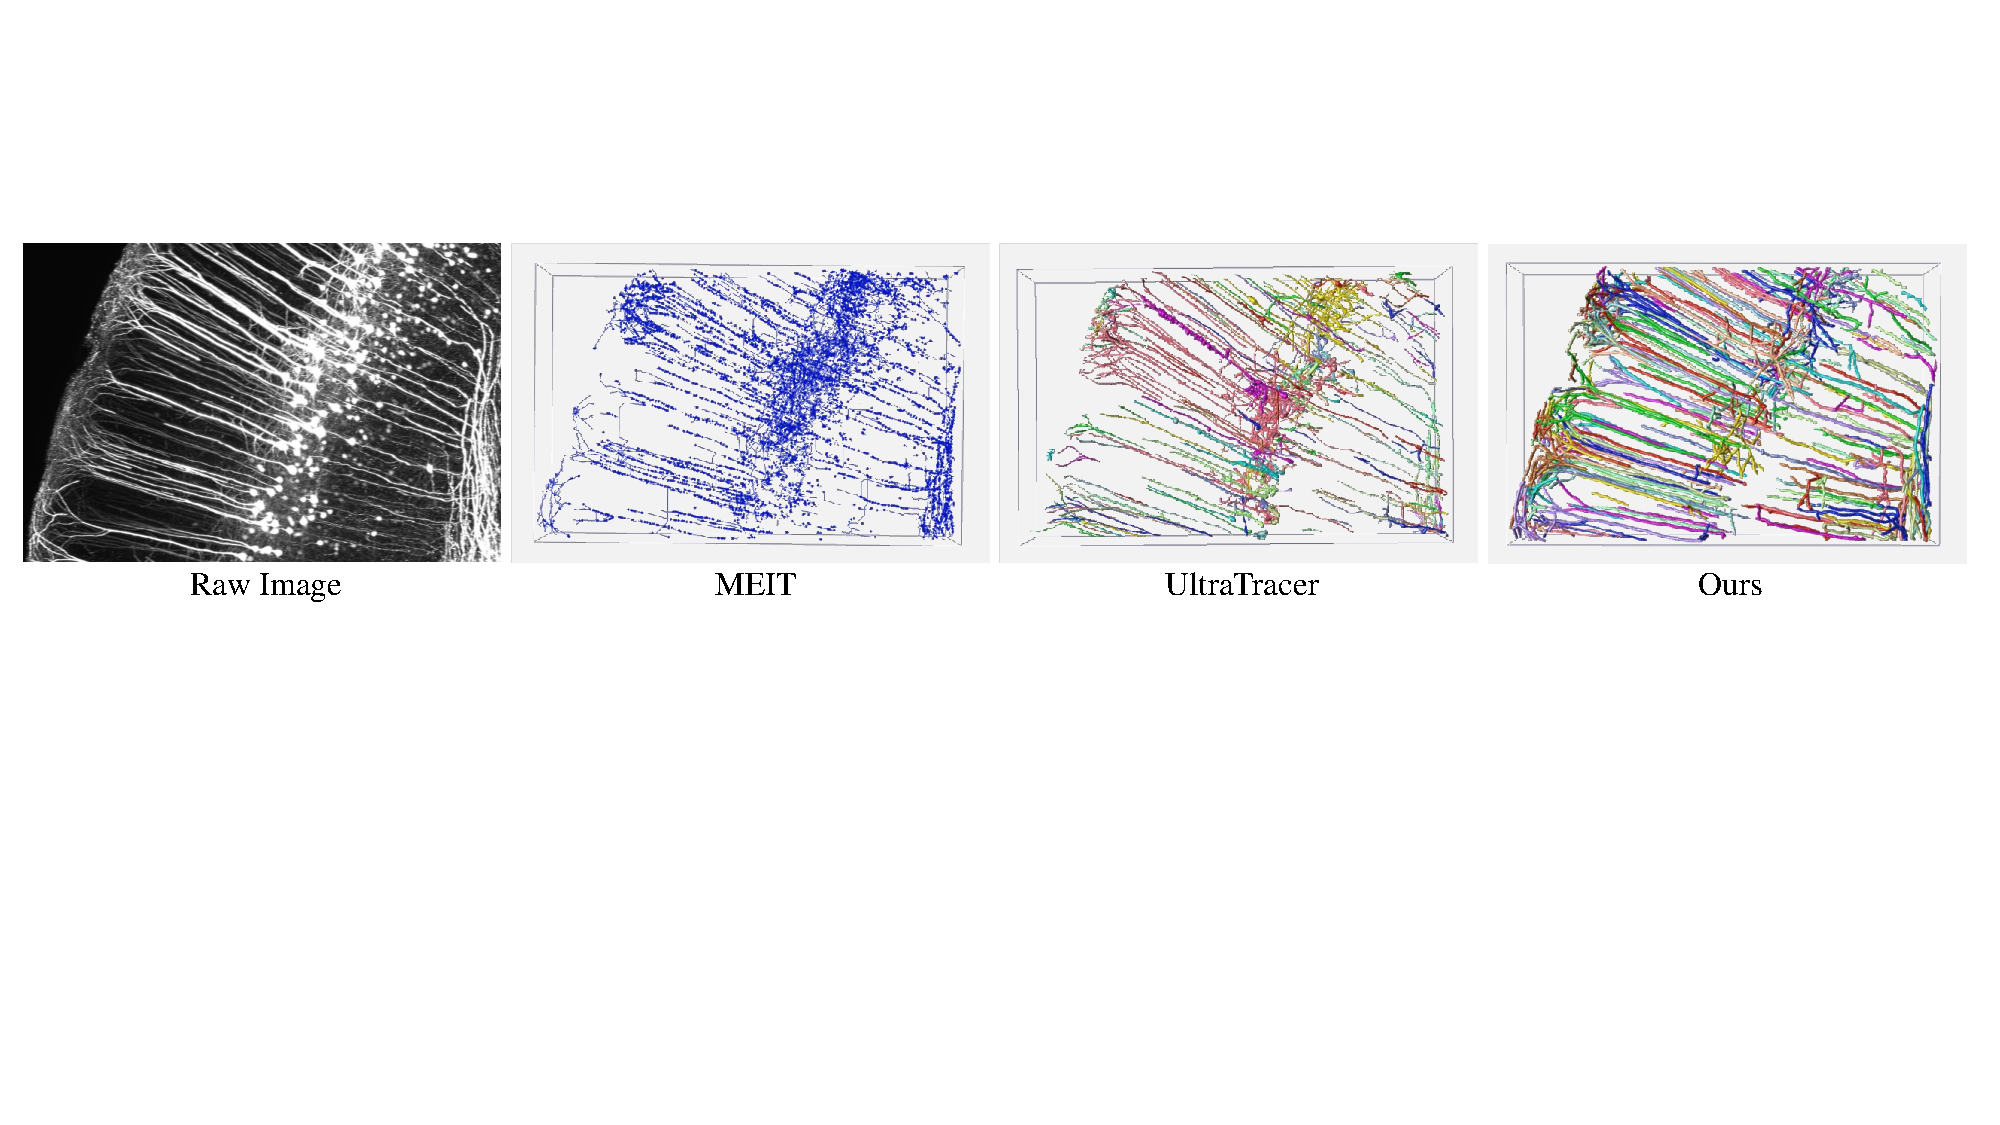
\includegraphics[width=\textwidth]{./Illustrations/comparison_ultranpr.pdf}
	\caption{Reconstruction results of dense neuronal populations from four adjacent large-scale blocks using UltraTracer~\cite{Peng2017}, MEIT~\cite{Wang2018} and our UltraNPR. \xj{The second row shows close-up views for a local region with dense neurites.} Our method reconstructs more complete and distinguishable neurons. 
	}
	\label{fig:reconstruct_blocks}
\end{figure*}



\begin{figure}[t]
	\centering
	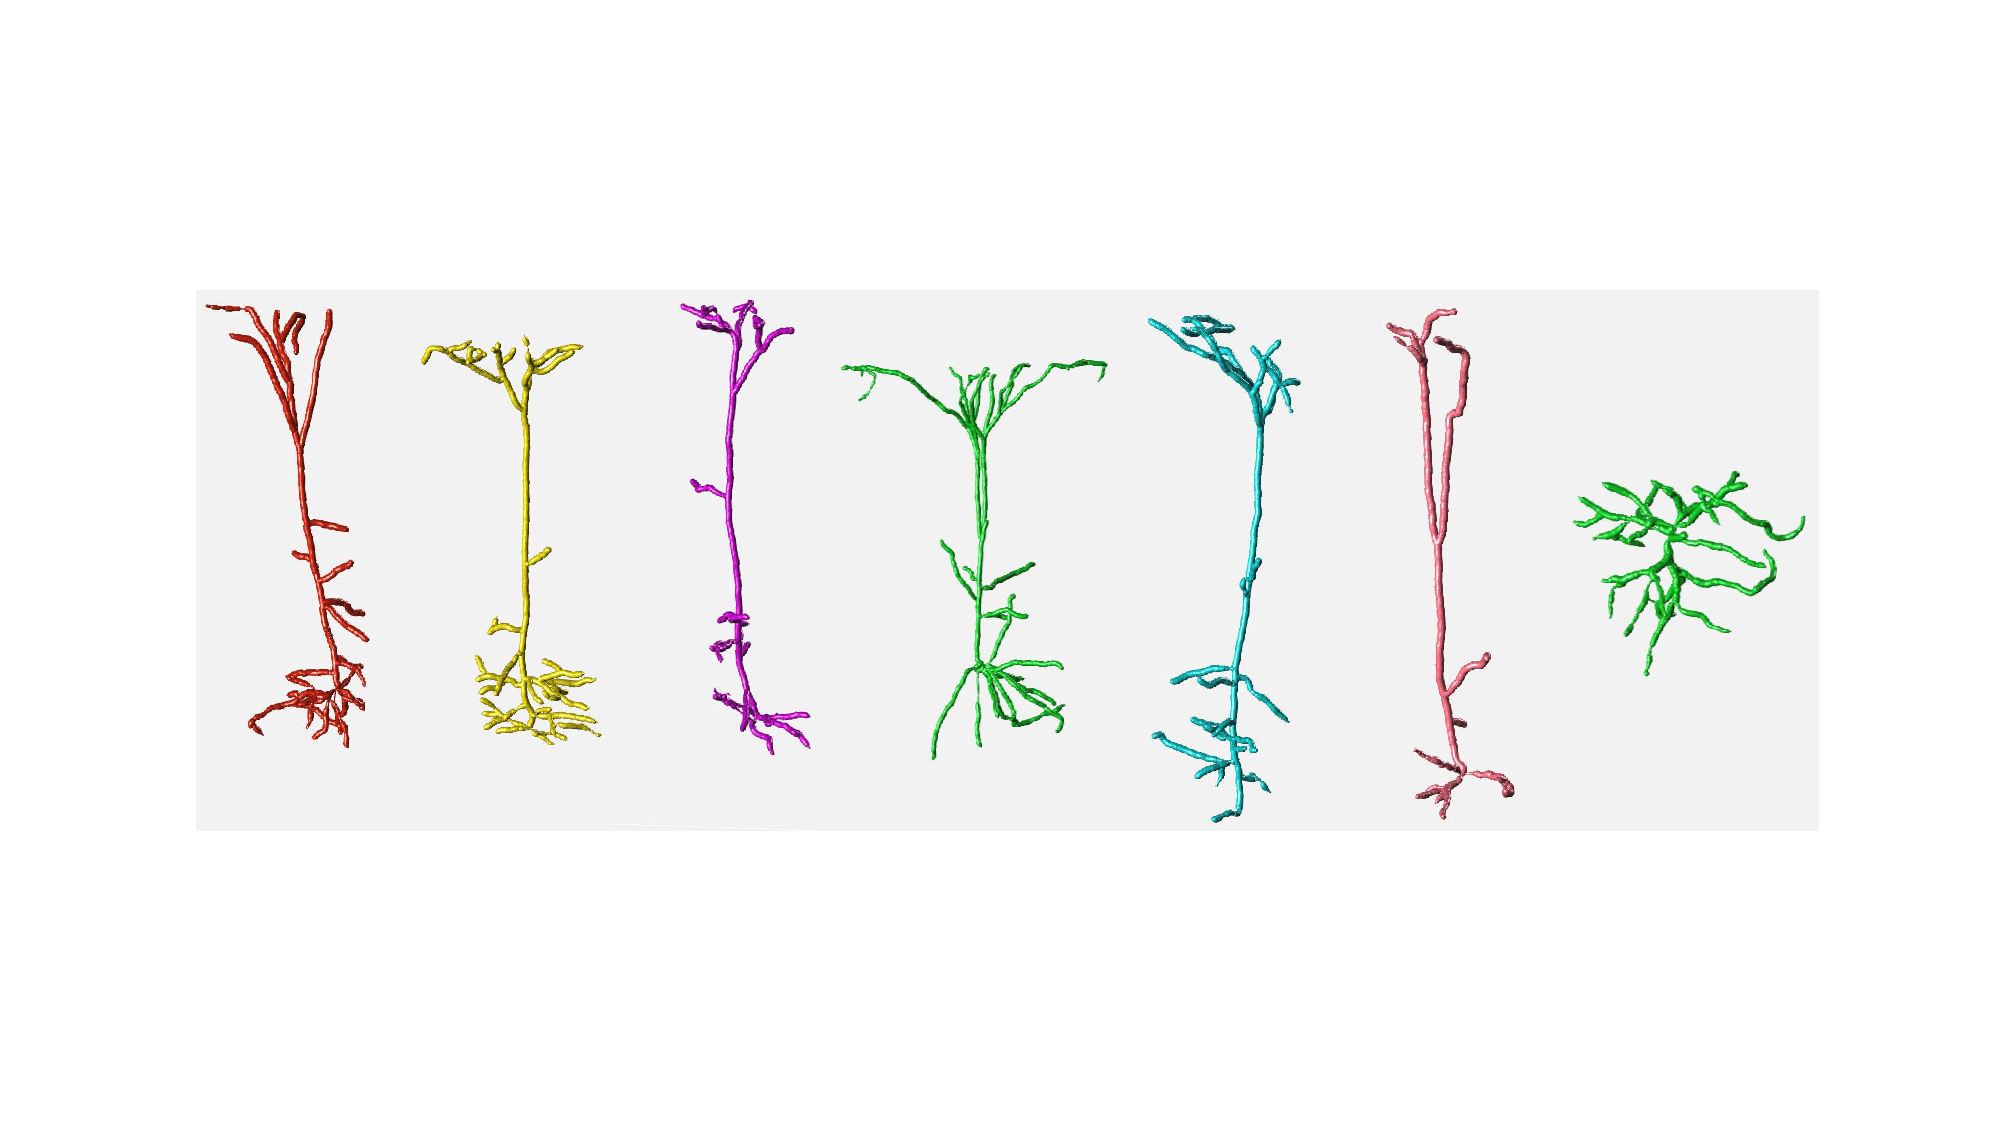
\includegraphics[width=\columnwidth]{./Illustrations/single_neurons4.pdf}
	\caption{Single neurons selected from the reconstructed neuronal populations in a mouse brain slice using our UltraNPR method.}
	\label{fig:single_neurons}
\end{figure}


Several neurons selected from the reconstructed neuronal population in the mouse brain slice are visualized in Fig.~\ref{fig:single_neurons}. 
We believe that these large-scale reconstructions provide detailed neuronal structures and will effectively support further neuronal morphology analysis in the whole brain. 
In summary, without any parameter-tuning and human interaction, our UltraNPR is capable of reconstructing dense neuronal populations from ultra-scale noisy OM images. 

